 %%%%%%%%%%%%%%%%%%%%%%%%%%%%%%%%%%%%%%%%%%%%%%%%%%%%%%%%%%%%%%%%%%%%%%
 %%%%%%%%%%%%%%%%%%%%%%%%%%%%%%%%%%%%%%%%%%%%%%%%%%%%%%%%%%%%%%%%%%%%%%
 %%%%                   Entity nodes
 %%%%%%%%%%%%%%%%%%%%%%%%%%%%%%%%%%%%%%%%%%%%%%%%%%%%%%%%%%%%%%%%%%%%%%
 %%%%%%%%%%%%%%%%%%%%%%%%%%%%%%%%%%%%%%%%%%%%%%%%%%%%%%%%%%%%%%%%%%%%%%
 
\section{Entity nodes}\label{sec:ENs}

\glyph{Entity nodes} (ENs) represent element of truth, class of things that exist. 
%In ontology parlance, they would be ``continuants''. 
Entity nodes are the source of \glyph{influences} (\sect{influences}). \SBGNERLone{} provides three different types of \glyph{entity nodes}, the \glyph{interactors}, the \glyph{logical operators} and the \glyph{perturbing agent}. 

\subsection{Interactors}\label{sec:interactors}

Interactors are entity nodes that are able to participate in an interaction (\sect{interaction}). \SBGNERLone{} provides two interactors, the \glyph{entity} and the \glyph{outcome} of a statement.

%%%%%%%%%%%%%%%%%%%%%%%%%%%%%%%%%%%%%%%%%%%%%%%%%%%%%%%%%%%%%%%%%%%%%%
%%                     Entity
%%%%%%%%%%%%%%%%%%%%%%%%%%%%%%%%%%%%%%%%%%%%%%%%%%%%%%%%%%%%%%%%%%%%%%
%\color{blue}

\subsubsection{Glyph: \glyph{Entity}}
\label{sec:entity}

\SBGNERLone defines only one glyph for all entities, whether physical entity, such as protein, a nucleic acid, metabolite or functional entity such as a gene. Indeed the exact nature of entities does not impact the rules of interactions within a map. The nature of a particular entity may then be clarified using its label and decorations, as will become clear below. 

\begin{glyphDescription}

\glyphSboTerm SBO:0000245 ! entity 

\glyphContainer An \glyph{entity} is represented by a rectangular container with rounded corners, as illustrated in \fig{ex-entity}.

\glyphLabel An \glyph{entity} is identified by a label placed in an unbordered box containing a string of characters.  The characters can be distributed on several lines to improve readability, although this is not mandatory.  The center of the label box must be located in the container. The label may spill outside of the container. 

\glyphAux An \glyph{entity} might carry state variables that can add information about its state (\sect{stateVariable}).  A state variable is represented by a ``stadium'', that is a rectangle capped with two hemi-circles. The center of the bounding box of \glyph{state variables} is located on the border and the long axis of this stadium is aligned with that part of the border of the \glyph{entity}'s container, as illustrated in \fig{ex-entity}.  The label of the state variable (which can precise the type of characteristic represented by the state variable, residue type, residue number etc.) is written within the state variable's container. Particular \glyph{state variables} are the existence (\sect{existence}) and the location (\sect{location}).

An \glyph{entity} can carry one or several \glyph{units of information} (\sect{unitInformation}).  Particular \glyph{units of information} are available for describing the material type (\sect{material-types-cv}) and the conceptual type (\sect{conceptual-types-cv}) of a macromolecule.  The center of the bounding box of a \glyph{unit of information} is located on the border and the long axis of this stadium is aligned with that part of the border of the \glyph{entity}'s container.

\end{glyphDescription}

%\begin{figure}[H]
%  \centering
%  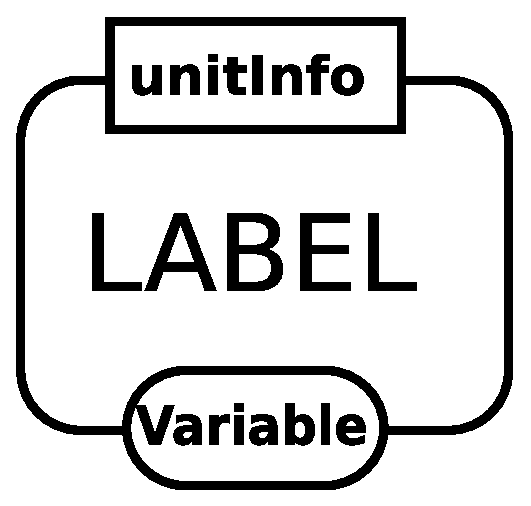
\includegraphics[scale = 0.3]{images/entity}
%  \caption{The \ER glyph for \glyph{entity}, showing a unit of information (\sect{unitInformation}), and two state variables (\sect{stateVariable}).}
%  \label{fig:entity}
%\end{figure}

\begin{figure}[H]
  \centering
  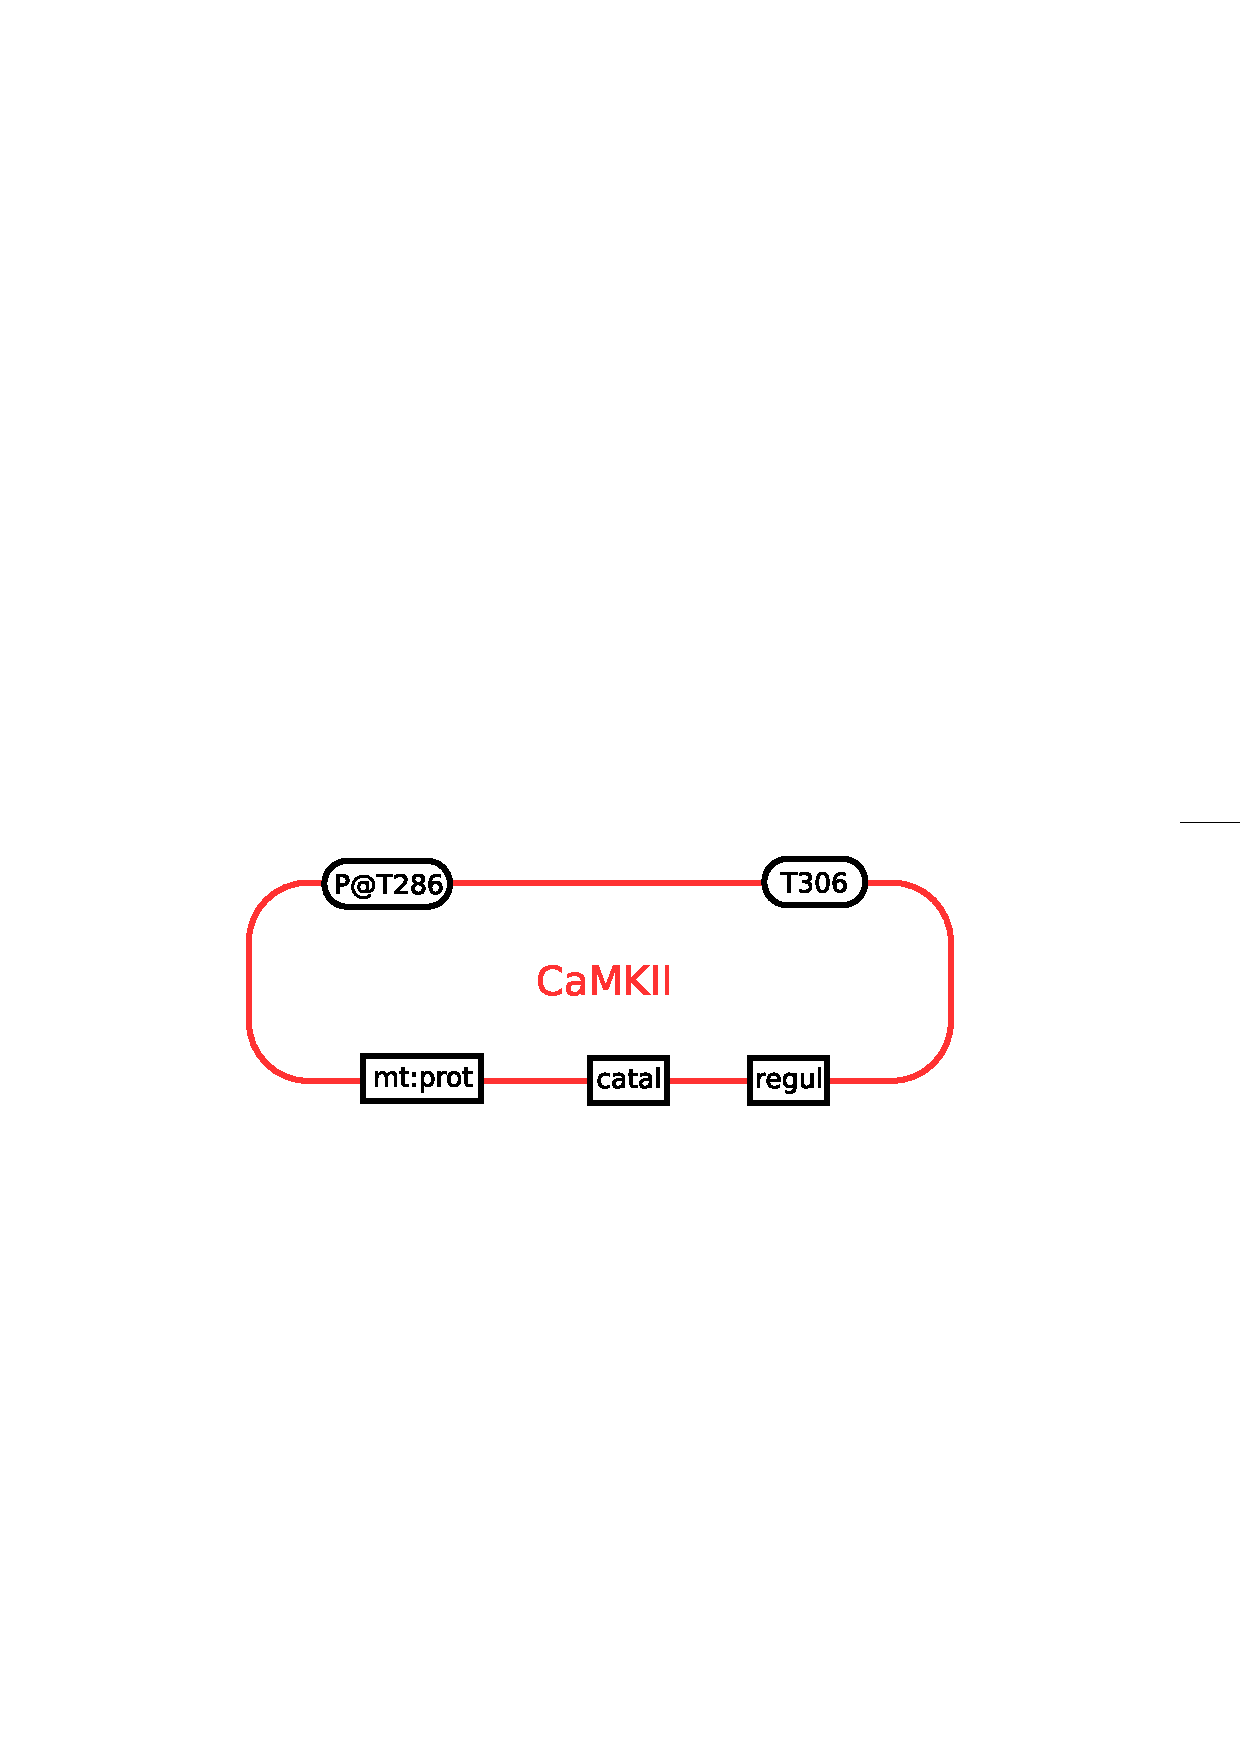
\includegraphics[scale = 0.5]{examples/ex-entity}
  \caption{Example of an \glyph{entity} named CaMKII, that carries two \glyph{state variables} representing the phosphorylated residue threonine 286 and the residue threonine 306, and a \glyph{unit of information} precising its material status (protein).}
  \label{fig:ex-entity}
\end{figure}

The granularity of the representation, that is what a given \glyph{entity} actually represents, is let to the person generating the map. For instance (\fig{entity-granularity}), one could choose to represent phosphorylated and non-phosphorylated forms of a protein using a single \glyph{entity}, carrying a \glyph{state variable} representing the phosphorylation. The phosphorylated form would be represented by the \glyph{outcome} located on the \glyph{assignment}. Alternatively one could create separate entity for phosphorylated state, carrying the \glyph{existence} \glyph{state variable} and represent phosphorylation by assignment of the true value to the \glyph{existence} \glyph{state variable}.

\begin{figure}[H]
  \centering
  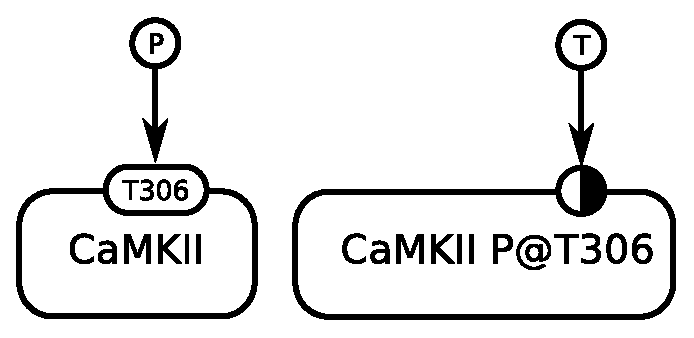
\includegraphics[scale = 0.5]{images/entity-granularity}
  \caption{The two ways to represent phosphorylation of the protein: by assigning ``P'' to the state variable (left), and by setting existence to phosphorylated \glyph{entity} (right).}
  \label{fig:entity-granularity}
\end{figure}

%\normalcolor


%%%%%%%%%%%%%%%%%%%%%%%%%%%%%%%%%%%%%%%%%%%%%%%%%%%%%%%%%%%%%%%%%%%%%%
%%%%                   Outcome
%%%%%%%%%%%%%%%%%%%%%%%%%%%%%%%%%%%%%%%%%%%%%%%%%%%%%%%%%%%%%%%%%%%%%%
\color{red}
\subsection{\glyph{Outcome}}\label{sec:outcome}

\subsubsection{Introduction}

In \ER, an \glyph{outcome} represents the result of an \glyph{interaction} (section \ref{sec:interaction}) or an \glyph{assignment} (\ref{sec:assignment}). For instance, if an \glyph{interaction} represents a non-covalent binding, the \glyph{outcome} represents the complex. If an \glyph{interaction} represents a genetic interaction, for instance derived from genetic screenings, the \glyph{outcome} represents the result of the presence of the two polymorphisms. If an \glyph{assignment} represents the phosphorylation of a protein, the \glyph{outcome} represents the phosphorylated form of this protein.

\begin{glyphDescription}

\glyphSboTerm SBO:0000409 ! interaction outcome

\glyphContainer  An \glyph{outcome} is represented by a black dot located on the arc of an \glyph{interaction} (see section~\ref{sec:interaction}) or an \glyph{assignment} (see section~\ref{sec:assignment}). The diameter of the dot has to be larger than the thickness of the arc.

\glyphLabel An \glyph{outcome} has no identity on its own and does not carry any label. 

\glyphAux An \glyph{outcome} does not carry any auxiliary items.

\end{glyphDescription}

\begin{figure}[H]
  \centering
  
\includegraphics[scale = 0.3, trim = 0 0 0 0.25in]{images/outcome}
  \caption{Examples of the \ER glyph for \glyph{outcome}.}
  \label{fig:outcome}
\end{figure}

\normalcolor
	


% %%%%%%%%%%%%%%%%%%%%%%%%%%%%%%%%%%%%%%%%%%%%%%%%%%%%%%%%%%%%%%%%%%%%%%
% %%%%%%%%%%%%%%%%%%%%%%%%%%%%%%%%%%%%%%%%%%%%%%%%%%%%%%%%%%%%%%%%%%%%%%
% %%%%                   Logical operators
% %%%%%%%%%%%%%%%%%%%%%%%%%%%%%%%%%%%%%%%%%%%%%%%%%%%%%%%%%%%%%%%%%%%%%%
% %%%%%%%%%%%%%%%%%%%%%%%%%%%%%%%%%%%%%%%%%%%%%%%%%%%%%%%%%%%%%%%%%%%%%%

\subsection{Logical operators}\label{sec:logic}

A \glyph{logical operator} allows to combine elements of truth into another element of truth (if A exists and B exits, then A AND B exists) in order ot apply influences. \SBGNERLone{} provides four \glyph{logical operators}, \glyph{and}, \glyph{or}, \glyph{not} and \glyph{delay}.

%%%%%%%%%%%%%%%%%%%%%%%%%%%%%%%%%%%%%%%%%%%%%%%%%%%%%%%%%%%%%%%%%%%%%%
%%                     And
%%%%%%%%%%%%%%%%%%%%%%%%%%%%%%%%%%%%%%%%%%%%%%%%%%%%%%%%%%%%%%%%%%%%%%
\color{blue}
\subsection{Glyph: \glyph{And}}\label{sec:delay}

The glyph \glyph{and} is used to denote that all the \glyph{EPNs} linked as input are necessary to produce the output influence.  

\begin{glyphDescription}
 \glyphSboTerm SBO:0000173 ! and.
 \glyphOrigin One interactor (section~\ref{sec:interactors}) or logical operator (section~\ref{sec:logic}).
 \glyphTarget  One modulation (section~\ref{sec:modulation}), stimulation (section~\ref{sec:stimulation}), inhibition (section~\ref{sec:inhibition}), necessary  stimulation (section~\ref{sec:necessaryStimulation}), or absolute inhibition (section~\ref{sec:absoluteInhibition}) arc.
 \glyphNode \glyph{Not} is represented by a circle carrying the word  ``AND''.
\end{glyphDescription}

\begin{figure}[H]
  \centering
  \includegraphics[scale = 0.5]{images/and}
  \caption{The \ER glyph for \glyph{and}. Only two inputs are represented, but more would be allowed.}
  \label{fig:and}
\end{figure}


% The following diagrams illustrate the dephosphorylation of the MAP inase ERK by the protein phosphatase 2A and the STriatal Enriched Phosphatase, in ST (left) and ER (right). 
% 
% \begin{center}
% \scalebox{0.5}{\includegraphics{images/stimulation-example1}}
% \end{center}
\normalcolor

%%%%%%%%%%%%%%%%%%%%%%%%%%%%%%%%%%%%%%%%%%%%%%%%%%%%%%%%%%%%%%%%%%%%%%
%%                     Or
%%%%%%%%%%%%%%%%%%%%%%%%%%%%%%%%%%%%%%%%%%%%%%%%%%%%%%%%%%%%%%%%%%%%%%
%\color{blue}
\subsubsection{Glyph: \glyph{Or}}\label{sec:or}

The glyph \glyph{or} is used to denote that any of the \glyph{interactors} linked as input is sufficient to produce the output influence.

\begin{glyphDescription}

 \glyphSboTerm SBO:0000174 ! or.

 \glyphContainer \glyph{Or} is represented by a circle, with two connectors located at the opposite side for inputs and output.

  \glyphLabel \glyph{Or} is identified by the label ``OR'' placed in an unbordered box attached to the center of the container. 

  \glyphAux \glyph{Or} does not carry any auxiliary items.

\end{glyphDescription}

\begin{figure}[H]
  \centering
  \includegraphics[scale = 0.5]{images/or}
  \caption{The \ER glyph for \glyph{or}. Three inputs are represented, but two or more than three would be allowed.}
  \label{fig:or}
\end{figure}


\begin{figure}[H]
  \centering
  \includegraphics[scale = 0.5]{examples/ex-or}
  \caption{Example of the \glyph{or} logical operator, showing that either the dimerisation of CaMKII or its binding to Calmodulin preclude the phosphorylation of threonin 306.}
  \label{fig:ex-or}
\end{figure}
%%%%%%%%%%%%%%%%%%%%%%%%%%%%%%%%%%%%%%%%%%%%%%%%%%%%%%%%%%%%%%%%%%%%%%
%%                     Not
%%%%%%%%%%%%%%%%%%%%%%%%%%%%%%%%%%%%%%%%%%%%%%%%%%%%%%%%%%%%%%%%%%%%%%
%\color{blue}
\subsection{Glyph: \glyph{Not}}\label{sec:not}

The glyph \glyph{not} is used to denote that the \glyph{interactor} linked as input .....

\question{NLN}{I am not sure what it means actually} 

\begin{glyphDescription}
 \glyphSboTerm SBO:0000238 ! not.
 \glyphOrigin One interactor (section~\ref{sec:interactors}) or logical operator (section~\ref{sec:logic}).
 \glyphTarget  One modulation (section~\ref{sec:modulation}), stimulation (section~\ref{sec:stimulation}), inhibition (section~\ref{sec:inhibition}), necessary  stimulation (section~\ref{sec:necessaryStimulation}), or absolute inhibition (section~\ref{sec:absoluteInhibition}) arc.
 \glyphNode \glyph{Not} is represented by a circle carrying the word ``NOT''.
 \end{glyphDescription}

\begin{figure}[H]
  \centering
  \includegraphics[scale = 0.5]{images/not}
  \caption{The \PD glyph for \glyph{not}.}
  \label{fig:not}
\end{figure}


%%%%%%%%%%%%%%%%%%%%%%%%%%%%%%%%%%%%%%%%%%%%%%%%%%%%%%%%%%%%%%%%%%%%%%%
%%                     delay
%%%%%%%%%%%%%%%%%%%%%%%%%%%%%%%%%%%%%%%%%%%%%%%%%%%%%%%%%%%%%%%%%%%%%%
\color{red}
\subsubsection{Glyph: \glyph{delay}}\label{sec:delay}

The glyph \glyph{delay} is used to denote that the \glyph{interactor} linked as input does not produce the influence immediately.

\begin{glyphDescription}

 \glyphSboTerm SBO:NEW ! delay.

 \glyphContainer \glyph{Delay} is represented by a circle, with two connectors located at the opposite side for input and output.

  \glyphLabel \glyph{Delay} is identified by the greek letter ``$\tau$`` (``TAU'') placed in an unbordered box attached to the center of the container. 

  \glyphAux \glyph{Delay} does not carry any auxiliary items.

\end{glyphDescription}

\begin{figure}[H]
  \centering
  \includegraphics[scale = 0.5]{images/delay}
  \caption{The \ER glyph for \glyph{delay}.}
  \label{fig:delay}
\end{figure}
\normalcolor


% %%%%%%%%%%%%%%%%%%%%%%%%%%%%%%%%%%%%%%%%%%%%%%%%%%%%%%%%%%%%%%%%%%%%%%
% %%%%%%%%%%%%%%%%%%%%%%%%%%%%%%%%%%%%%%%%%%%%%%%%%%%%%%%%%%%%%%%%%%%%%%
% %%%%                   Perturbing agent
% %%%%%%%%%%%%%%%%%%%%%%%%%%%%%%%%%%%%%%%%%%%%%%%%%%%%%%%%%%%%%%%%%%%%%%
% %%%%%%%%%%%%%%%%%%%%%%%%%%%%%%%%%%%%%%%%%%%%%%%%%%%%%%%%%%%%%%%%%%%%%%

\subsection{Glyph: \glyph{Perturbing agent}}\label{sec:perturbation}
%%%%%%%%%%%%%%%%%%%%%%%%%%%%%%%%%%%%%%%%%%%%%%%%%%%%%%%%%%%%%%%%%%%%%%
%%                     Perturbing agent
%%%%%%%%%%%%%%%%%%%%%%%%%%%%%%%%%%%%%%%%%%%%%%%%%%%%%%%%%%%%%%%%%%%%%%
\color{red}

\subsection{Glyph: \glyph{Perturbing agent}}
\label{sec:perturbation}
 
Biochemical networks can be affected by external influences. Those
influences can be well-defined physical perturbations, such as a the effect of a light
pulse or of a change in temperature; they can also be more complex and not
well-defined phenomena, for instance a biological process, an experimental
setup, or a mutation.  For these situations, SBGN provides the
\glyph{perturbing agent} glyph. We do not use the word \emph{perturbation} to avoid the misunderstanding with the influence that the \glyph{perturbing agent} has on the map. 

\begin{glyphDescription}

\glyphSboTerm SBO:0000405 ! perturbing agent

\glyphContainer A \glyph{perturbing agent} is represented by a modified hexagon
having two opposite concave faces, as illustrated in \fig{perturbation}.

\glyphLabel A \glyph{perturbing agent} is identified by a label placed in an
unbordered box containing a string of characters.  The characters can be
distributed on several lines to improve readability, although this is not
mandatory.  The label box must be attached to the center of the
\glyph{perturbing agent} container.  The label may spill outside of the container.

\glyphAux A \glyph{perturbing agent} does not carry any auxiliary unit. [DOES-IT NOT? IS-IT AN ENTRY POINT? WHAT ABOUT THE EXISTENCE AND LOCATION VARIABLES?]

\end{glyphDescription}

\begin{figure}[H]
  \centering
  \includegraphics[scale = 0.3]{images/perturbation}
  \caption{The \ER glyph for \glyph{perturbing agent}.}
  \label{fig:perturbation}
\end{figure}

\normalcolor
